\section{Related Work}

\subsection{CountMin}

CountMin\cite{cormode_improved_2003} is a 2-dimensional data structure that is used for frequency approximation queries. It has a width of \(w = \ceil{e / \epsilon}\) and a depth of \(d = \ceil{ln(1 / \delta)}\). Here the \(e\) is the base of the natural logarithm while \(\epsilon\) and \(\delta\) are user-specified constants. The underlying idea is to hash the aggregated frequencies of the edges using multiple hash functions into predefined blocks, as indicated in Fig.~\ref{fig:countmin}. Any incoming edge \(e_t\) at timestamp \(t\) will get hashed into each row using its hash function \(h_d\). A CountMin sketch will have a fixed memory allocation of \(w \cdot d\) throughout its lifespan. Irrespective of the volume of the data stored in the sketch, the initial memory allocation will not change. Thus the accuracy of the queries will decrease as more and more data is inserted into the sketch. Despite the weaknesses, CountMin can be considered as a good generalized summarization sketch as many other current techniques are geared towards specific graph computation scenarios. However, the CountMin approach is not restricted to streaming graphs but other applications as well\cite{cormode_improved_2003}. 

\begin{figure}[htbp]
    \centerline{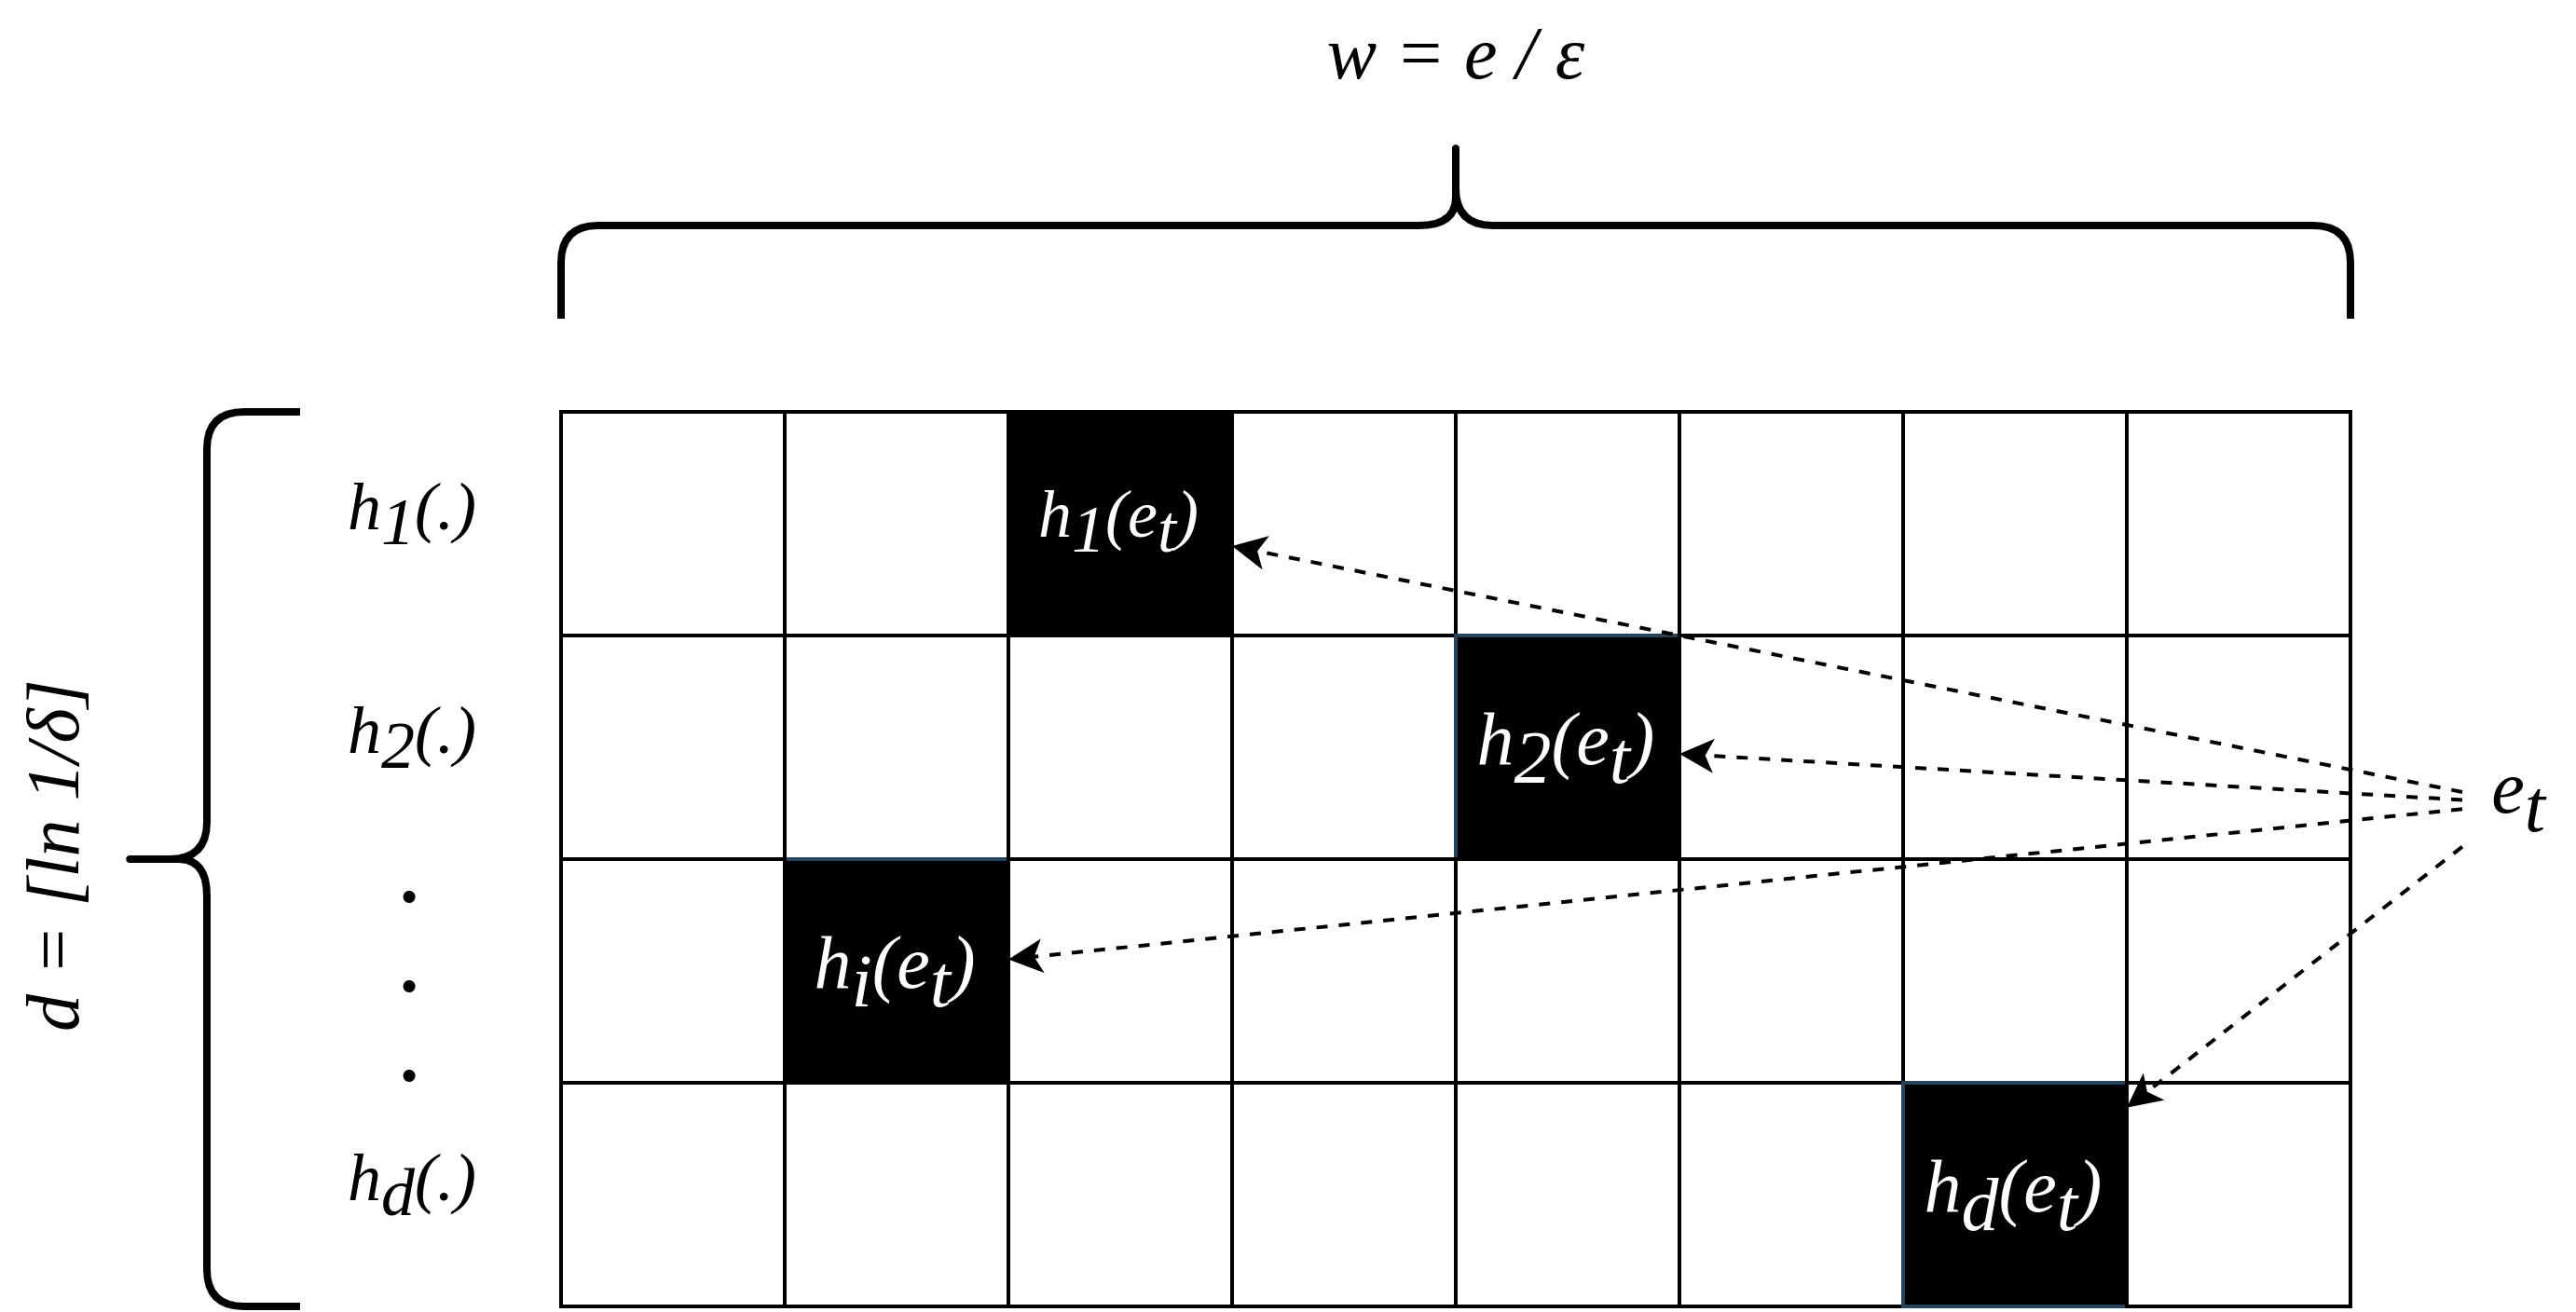
\includegraphics[width=0.5\textwidth]{img/countmin.png}}
    \caption{CountMin sketch\cite{zhao_gsketch:_2011}}
    \label{fig:countmin}
\end{figure}

\subsection{gSketch}

gSketch\cite{zhao_gsketch:_2011} is an extension of CountMin data structure. But unlike the CountMin sketch, this is specifically geared towards summarizing graph streams. gSketch is based on one of the below two assumptions.

\begin{itemize}
    \item A sample of the graph stream is available.
    \item Samples of both the graph stream and the query workload are available.
\end{itemize}

In CountMin, one global sketch is created for the entire stream. By doing so, it fails to take advantage of any structural properties present in the graph stream. gSketch tries to avoid this by considering the underlying structure of the graph stream using a sample. It then proceeds to partition its allocated space, as indicated in Fig.~\ref{fig:gsketch}. The goal of this partitioning step aims to maintain a sufficient frequency uniformity within each localized sketch in a way such that the combined error of the quarry estimations over the entire graph is kept at a minimum.

\begin{figure}[htbp]
    \centerline{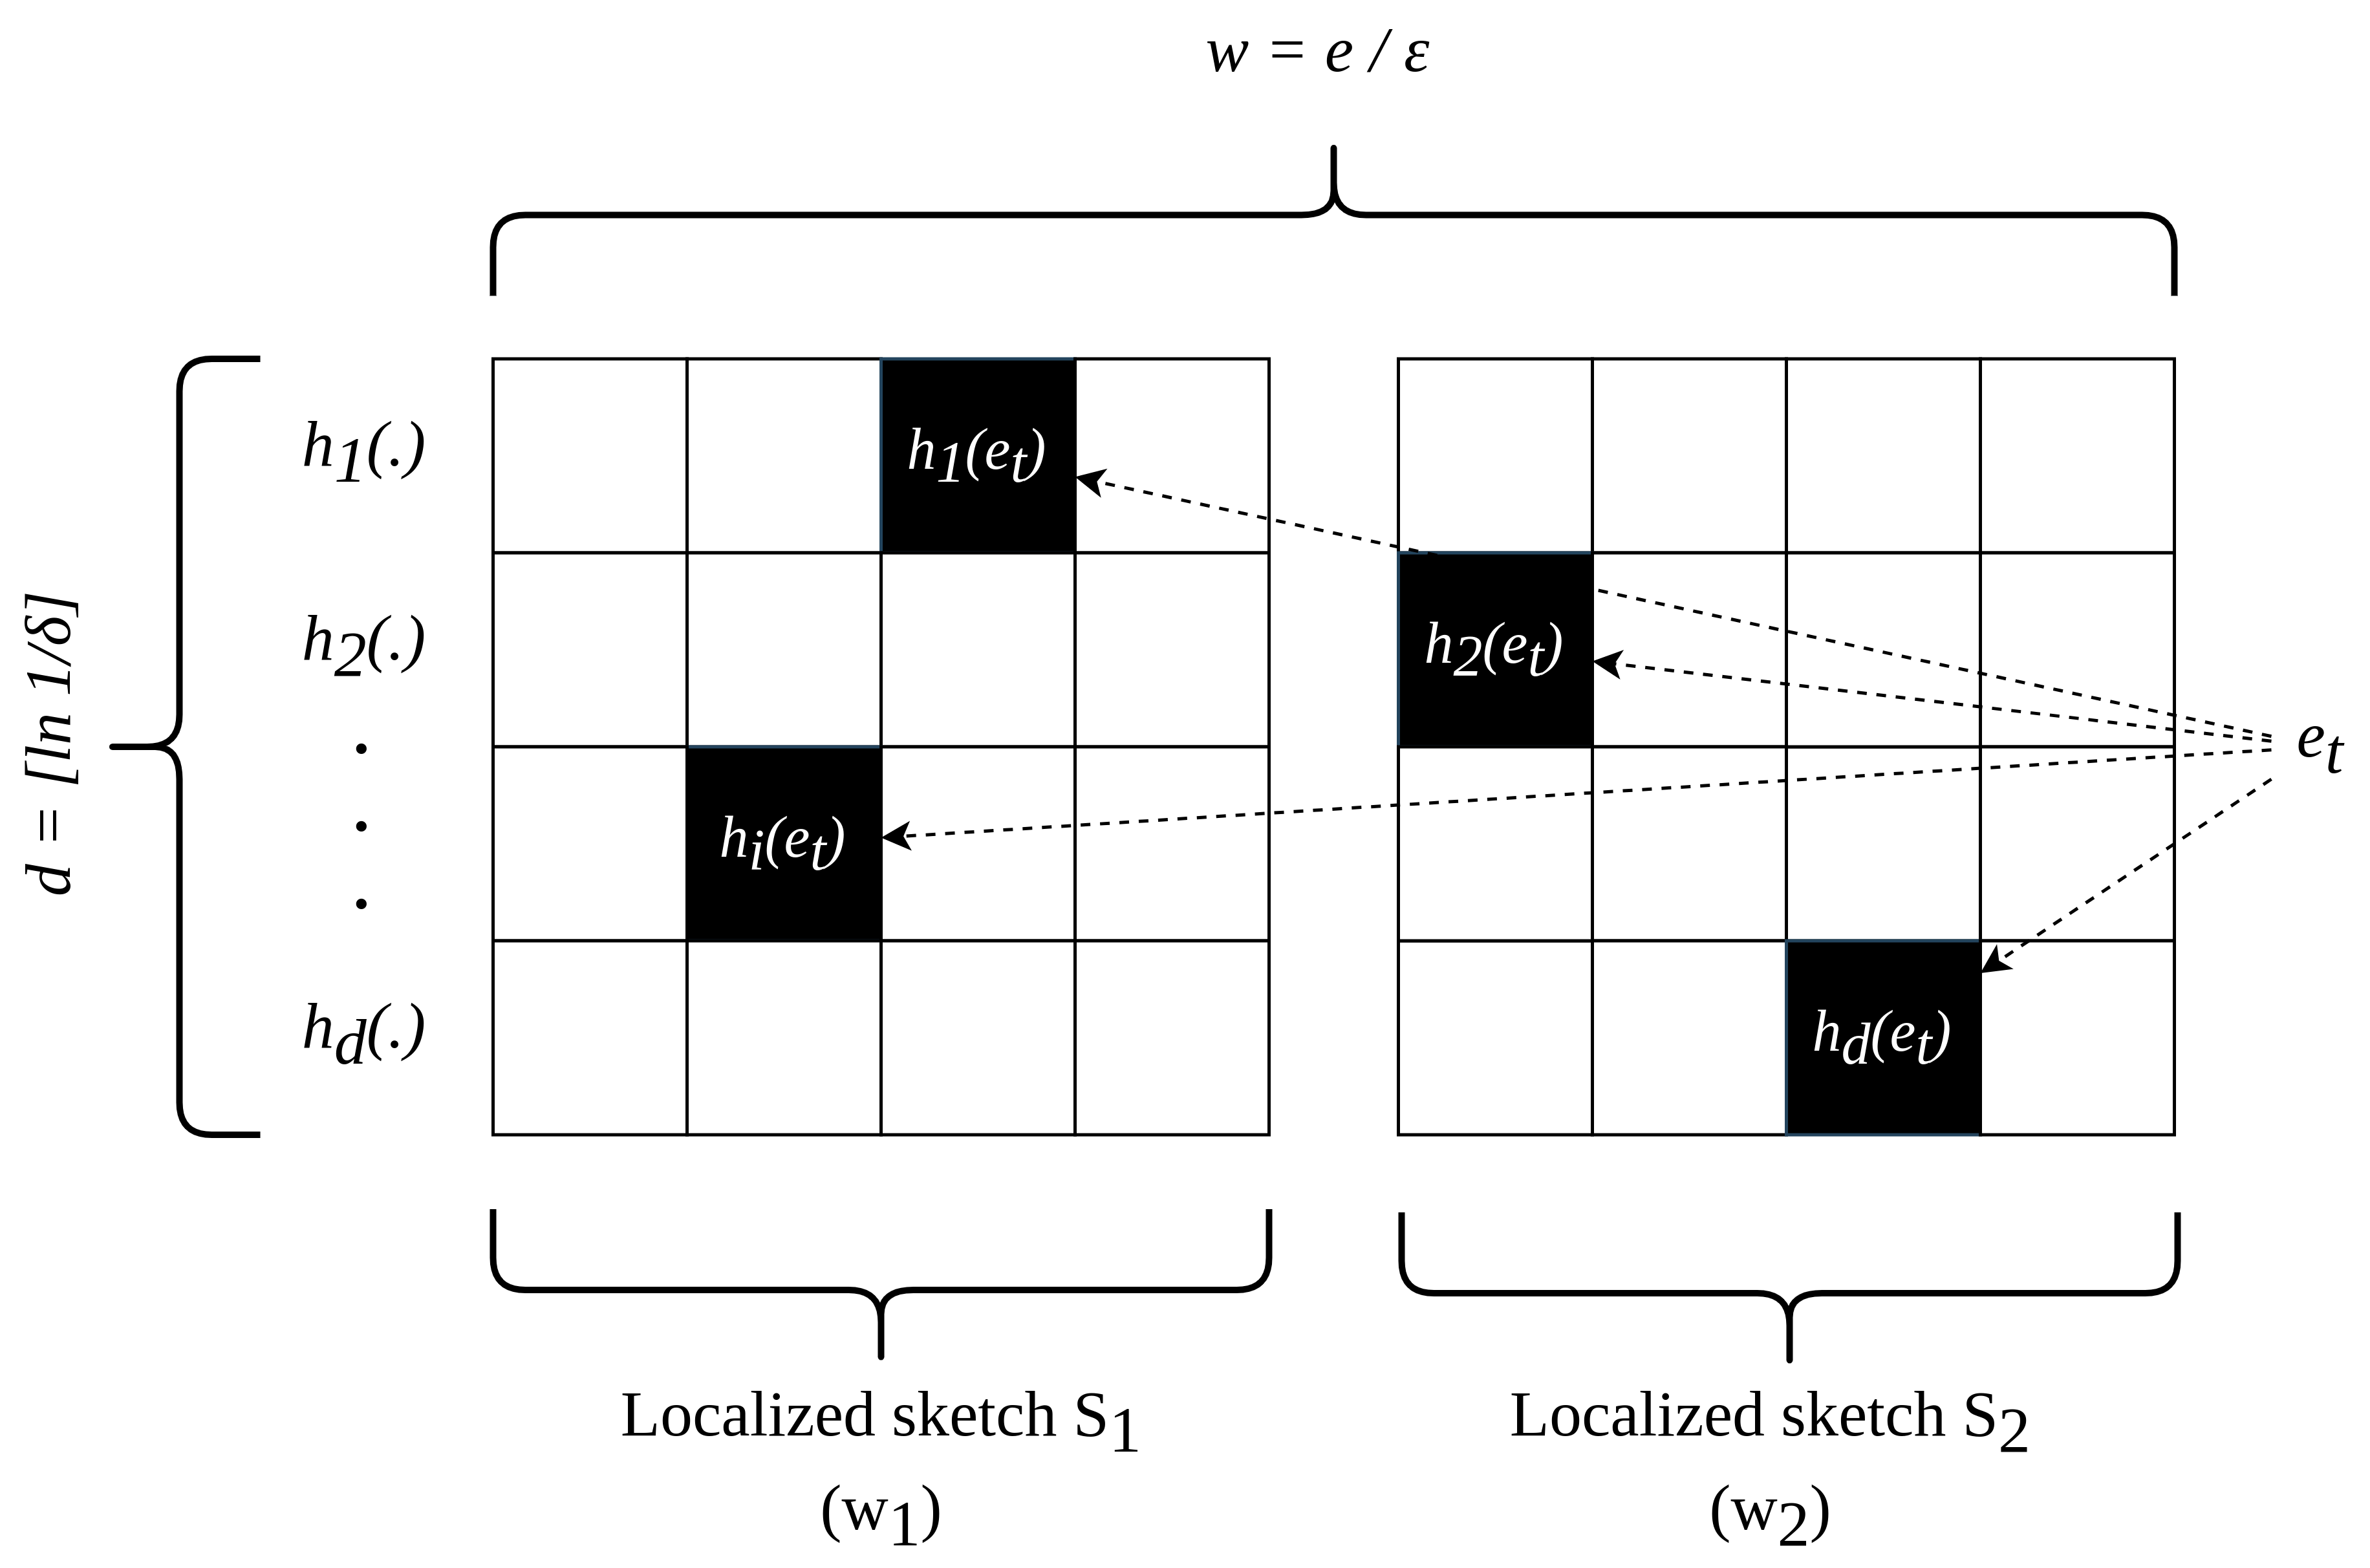
\includegraphics[width=0.5\textwidth]{img/gsketch.png}}
    \caption{gSketch sketch}
    \label{fig:gsketch}
\end{figure}

\subsection{TCM}

A disadvantage posed by all the approximate frequency count sketches like CountMin or gSketch is that they do not store the locality of the nodes. Therefore CountMin and gSketch cannot be used for conditional node queries or queries involving node connectivity. If these queries were to be run, the locality of the nodes has to be retained in the graph synopses. TCM\cite{tang_graph_2016} aims to solve this issue by storing the connectivity of the nodes in its data structure. TCM can summarize both node and edge information in constant time. Thus, it can answer a wide range of queries, unlike its predecessors. The structure of a TCM sketch is depicted in Fig.~\ref{fig:tcm}. TCM sketch could be considered as one of the pioneering works in summarizing data streams, which is directly related to our work presented in this paper.

\begin{figure}[htbp]
    \centerline{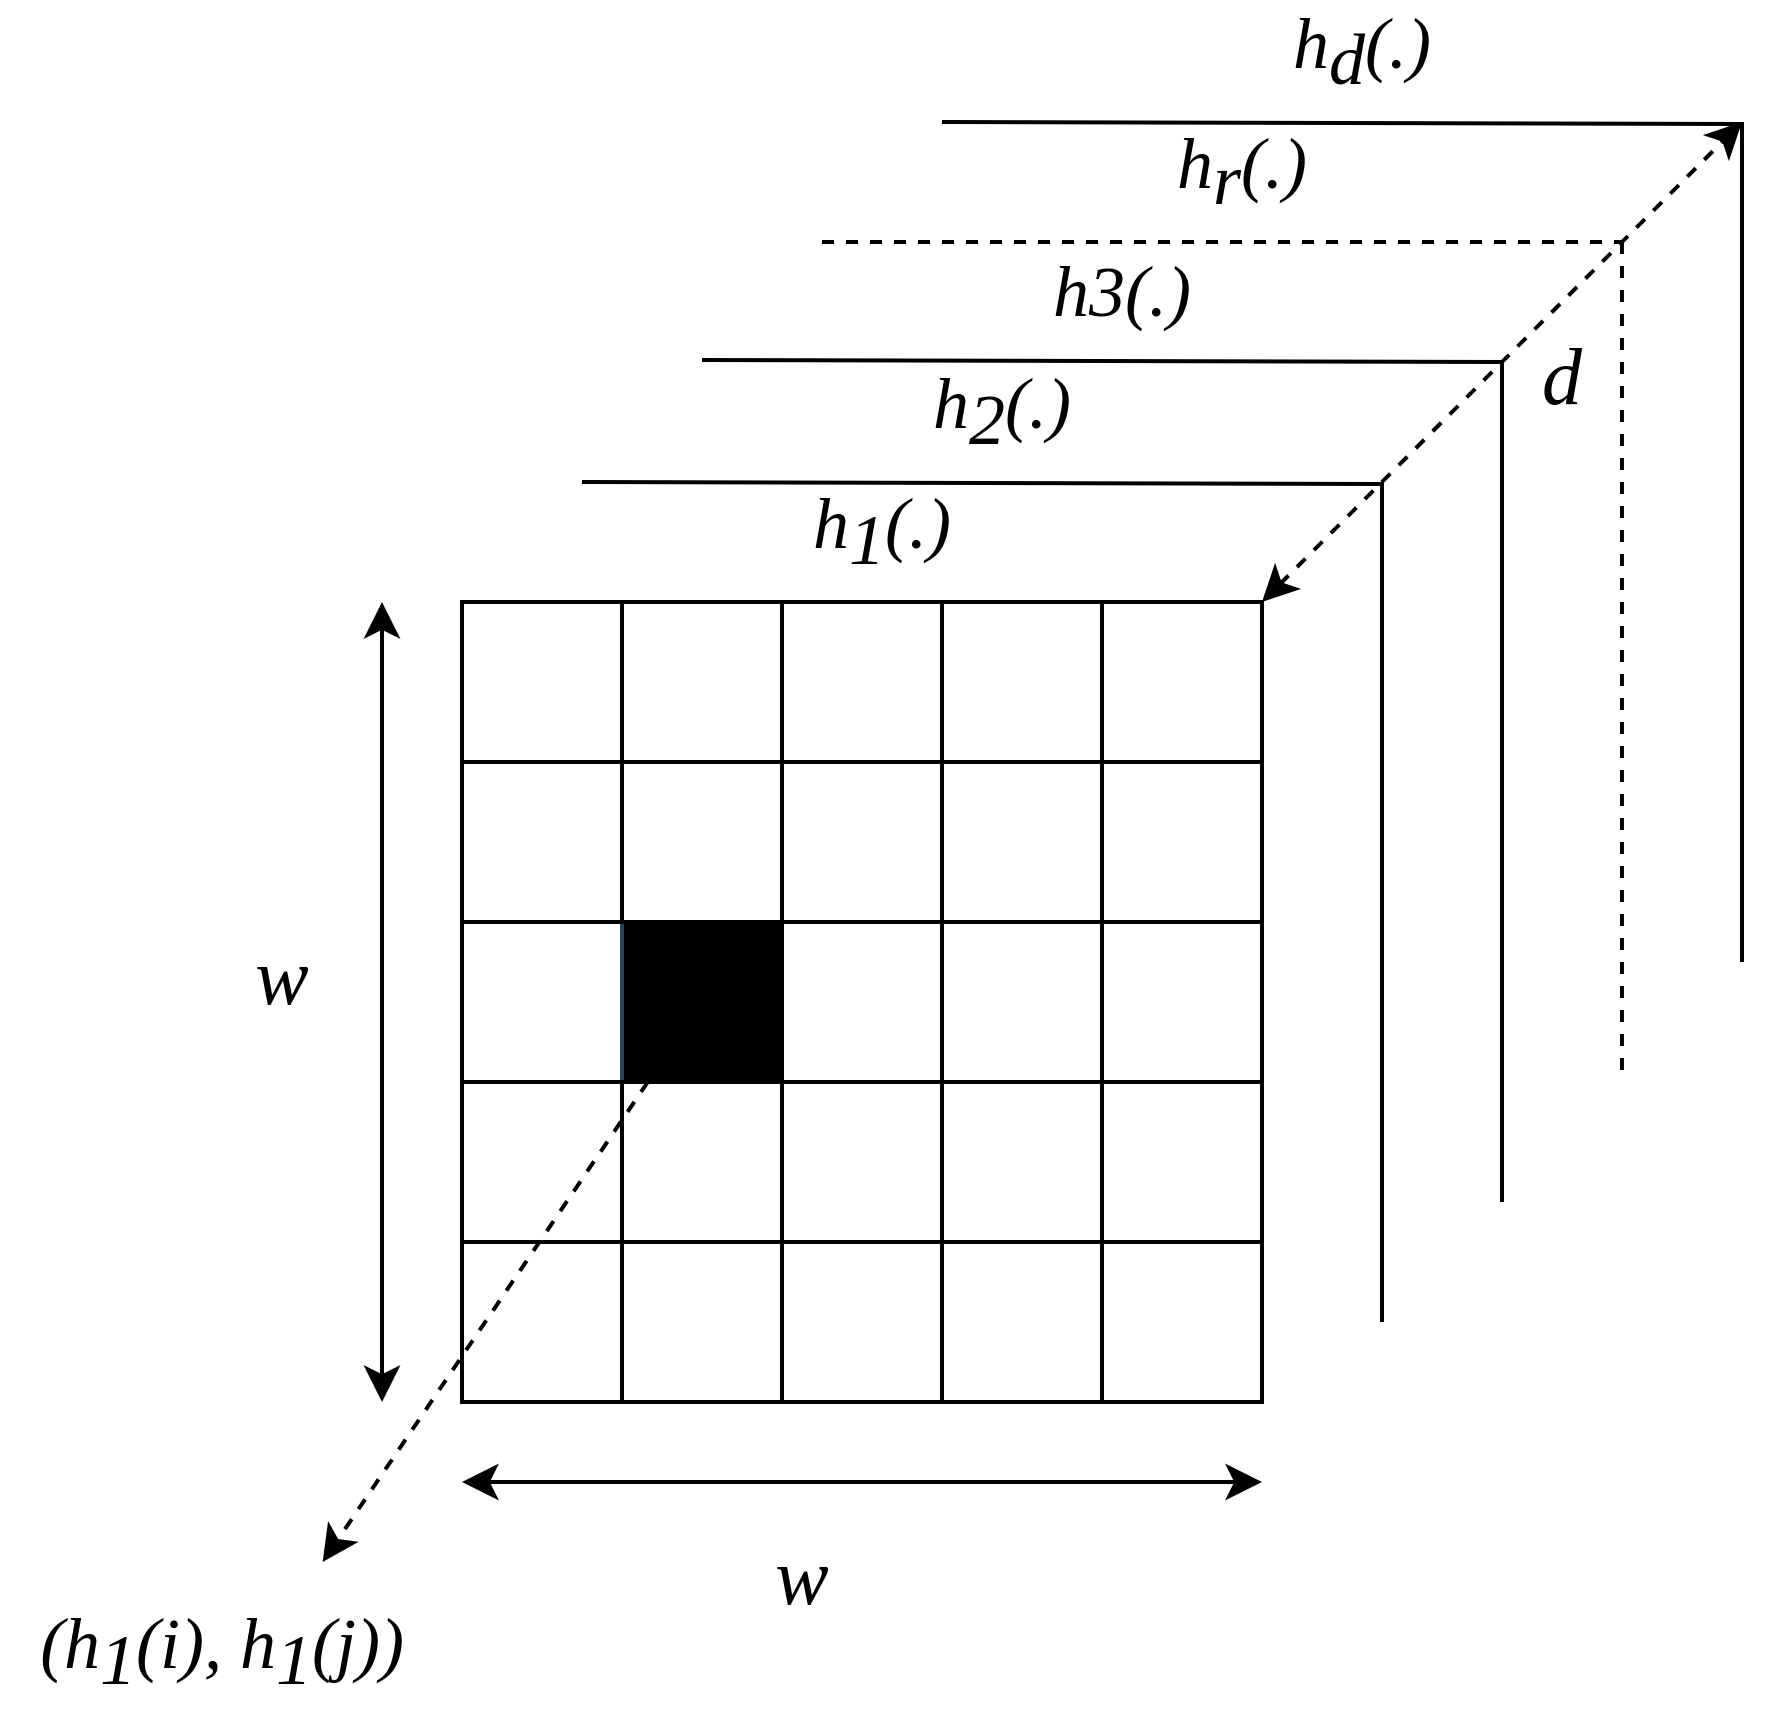
\includegraphics[width=0.35\textwidth]{img/tcm.png}}
    \caption{TCM sketch\cite{khan_query-friendly_2016}}
    \label{fig:tcm}
\end{figure}

\subsection{gMatrix}

The functionality of gMatrix\cite{khan_query-friendly_2016} is very similar to the TCM sketch. However, gMatrix considers several aspects which the TCM sketch does not address.

\begin{itemize}
    \item Reverse hashing queries through pairwise independent hash functions.
    \item Alternative options to extend sketch and space-saving synopses.
\end{itemize}
